\typeout{}\typeout{If latex fails to find aiaa-tc, read the README file!}

\documentclass[]{aiaa-tc}% insert '[draft]' option to show overfull boxes
\usepackage{graphicx}
\usepackage{array}
\usepackage{setspace}
\usepackage{overcite}
\usepackage{lastpage}
\usepackage{fancyhdr}
\usepackage{subcaption}
\usepackage{gensymb}
\usepackage{amssymb}
\usepackage{amsfonts}
\usepackage{amstext}
\usepackage{amsmath}

 \title{Autonomous Optical Navigation for Earth-Observing Satellites Using Coastline Matching}

 \author{
  Miranda N. Straub%
    \thanks{Graduate Research Assistant, Department of Mechanical and Aerospace Engineering, Benjamin M. Statler College of Engineering and Mineral Resources.}
  \ and John A. Christian%
	\thanks{Assistant Professor, Department of Mechanical and Aerospace Engineering, Benjamin M. Statler College of Engineering and Mineral Resources, and AIAA Senior Member.}\\
  {\normalsize\itshape
  West Virginia University, Morgantown, WV, 26506}
 }

 % Data used by 'handcarry' option if invoked
 \AIAApapernumber{2015}
 \AIAAconference{SciTech, January 5-9, and Kissimmee, FL}
 \AIAAcopyright{\AIAAcopyrightD{2015}}

 % Define commands to assure consistent treatment throughout document
 \newcommand{\eqnref}[1]{(\ref{#1})}
 \newcommand{\class}[1]{\texttt{#1}}
 \newcommand{\package}[1]{\texttt{#1}}
 \newcommand{\file}[1]{\texttt{#1}}
 \newcommand{\BibTeX}{\textsc{Bib}\TeX}

\begin{document}

\maketitle

\begin{abstract}
In order to meet the demands of future space missions, it is beneficial for spacecraft to have the capability to support autonomous navigation. This is true for both crewed and uncrewed vehicles. For crewed vehicles, autonomous navigation would allow the crew to safely navigate home in the event of a communication system failure. For uncrewed missions, autonomous navigation reduces the demand on ground-based infrastructure and could allow for more flexible operation. One promising technique for achieving these goals is through optical navigation. To this end, the present work considers how camera images of the Earth's surface could enable autonomous navigation of a satellite in low Earth orbit. Specifically, this study will investigate the use of coastlines and other natural land-water boundaries for navigation. Observed coastlines can be matched to a pre-existing coastline database in order to determine the location of the spacecraft. This paper examines how such measurements may be processed in an on-board Extended Kalman Filter (EKF) to provide completely autonomous estimates of the spacecraft state throughout the duration of the mission.
\end{abstract}

\section*{Nomenclature}

\begin{tabbing}
  XXX \= \kill% this line sets tab stop
  $\textbf{x}$ \> State Vector \\
  $\textbf{y}$ \> Measurement Vector \\
  $\textbf{P}$ \> State Covariance Matrix \\
  $\textbf{F}$ \> Jacobian Matrix \\
  $\textbf{Q}$ \> Process Noise Covariance Matrix \\
  $\textbf{H}$ \> Measurement Sensitivity Matrix \\
  $\textbf{K}$ \> Kalman Gain \\
  $\textbf{R}$ \> Measurement Covariance Matrix \\
  $\textbf{r}$ \> Spacecraft Position Vector \\
  $\textbf{s}$ \> Vector from spacecraft to observed landmark \\
  $\textbf{o}$ \> Vector from center of Earth to observed landmark \\
  $\textbf{e}$ \> Unit vector in direction of observed landmark \\
  $\textbf{T}$ \> Rotation Matrix \\
  $\mu$ \> Gravitational Parameter \\ [5pt]
 \end{tabbing}

%%%%%%%%%%%%%%%%%%%%%%%%%%%%%%%%%%%%%%%%%%%%%%%%%%%%%%%%
\section{Introduction}
With the many recent technological developments in the aerospace industry and the desire to conduct more ambitious space missions, there is an increasing need for fully autonomous spacecraft.  Autonomous spacecraft navigation systems are important for crewed and uncrewed missions.  In the case of crewed missions, autonomous navigation systems are crucial in bringing the crew home safely in case of a communication system failure.  For either scenario, previous work has shown optical navigation to be one method of fulfilling the need for autonomous navigation \cite{Christian:2012}.

The process of optical navigation includes capturing an image of a known object and using the information in this image to determine the location of the spacecraft.  Target bodies for optical navigation include planets, planetary satellites, asteroids, comets and stars \cite{Owen:2011}.  At closer ranges, surface features may be observed.  On Earth these surface features include coastlines, islands, and other in-land water boundaries such as lakes and rivers \cite{Liu:2004}.  Thus, the focus of this paper will be on autonomous optical navigation of a satellite in low-Earth orbit (LEO) using coastlines as landmarks.  

For this study, it is assumed that the only source of external measurements will be from a star-tracker (for attitude) and from an Earth-observing camera.  The state of the spacecraft will be propagated on-board using assumed dynamics and Inertial Measurement Unit (IMU) data.  In addition, a camera measurement model will be developed to utilize measurements obtained from landmark observations to be processed in an on-board Extended Kalman Filter (EKF).  These models will be discussed in detail later in the paper.

%%%%%%%%%%%%%%%%%%%%%%%%%%%%%%%%%%%%%%%%%%%%%%%%%%%%%%%%

\subsection{Navigation Using Landmarks}
Many studies have been carried out concerning the use of optical navigation with various surface landmarks as targets.  For example, craters commonly found on the surface of planets, satellites, asteroids, and other solar system bodies are often proposed as landmarks for optical navigation \cite{Cheng:2003,Rowell:2013,Hanak,Rohr:2011,Cheng:2003b}.  Generally, a crater can be identified in an image by looking for an elliptical rim and a bright to dark shading pattern depending on the lighting at the time of observation.  Because of these commonalities, most crater detection algorithms consist of a series of steps that include edge detection and ellipse fitting.  Once the ellipses are identified as landmarks, the size, shape, and position of that landmark relative to other landmarks are used to match the ellipses with a known database of craters for that body\cite{Hanak}.  It should be noted, however, that this process can be difficult because the craters often have different appearances when viewed from different directions and with different sun angles.  Also, the age of the crater may contribute to the sharpness of the crater edges on the surface which can make detection easier or more difficult \cite{Cheng:2003}. Techniques such as image cross-correlation, context based matching, and projective conic invariants can be used to make up for these differences but are beyond the scope of this paper. They are discussed in detail in [\citen{Cheng:2003}] and [\citen{Cheng:2003b}].

Due to the previously mentioned irregularities seen in crater detection, and because craters are less numerous on the Earth's surface, bodies of water can also be used as landmarks for spacecraft orbiting Earth in LEO.  This is easily observed due to the contrast in colors between land and water as seen by the spacecraft.  These bodies of water can include coastlines, islands, rivers, and lakes.  Additional features can be detected as well (e.g. volcanoes, mountains, snow, and even urban areas); however these are often changing over time and can be more difficult to distinguish and map \cite{SeenFromSpace}.

%%%%%%%%%%%%%%%%%%%%%%%%%%%%%%%%%%%%%%%%%%%%%%%%%%%%%%%%

\subsection{Coastline Determination}
Numerous methods of extracting coastlines from images have been studied.  Common solutions include using conventional image processing boundary detection methods or classifying illumination levels of an image.  When using boundary or edge detection, various methods are available and produce similar results depending on the situation.  One popular choice for edge detection is the Canny edge detector \cite{Canny:1986}.  Previous work by Liu and Jezek \cite{Liu:2004}, however, has shown Canny edge detection to be insufficient for coastline extraction due to the lack of consistent intensity contrast between land and water regions often resulting in discontinuous coastline data.  To alleviate this problem, image segmentation and post-segmentation processing were used in [\citen{Liu:2004}].  Other authors, such as those in [\citen{Heene:2000}], use two additional masking steps in addition to the Canny edge detection: an additional edge focusing step and a closing step used as an input for the object-oriented matching process.  These additional steps greatly helped automate the extraction of coastlines from the images used.

An additional problem that arises with coastline extraction and feature selection is the accuracy of determining actual coastlines.  For example, many edge detection techniques use contrast as a determining factor to differentiate boundaries and edges.  If the satellite image contains cloud coverage, it is possible for clouds to be considered boundaries and therefore identified as coastlines.  A solution to this problem was discussed in [\citen{Patt:1997}] using a global ocean color sensor which measures radiances in eight visible and near-infrared bands.  By creating scatter plots of radiance observed from two different bands, it was possible to normalize the data and specify thresholds to classify observed regions as land, water, clouds, or ice.  

%%%%%%%%%%%%%%%%%%%%%%%%%%%%%%%%%%%%%%%%%%%%%%%%%%%%%%%%

\subsection{Georeferenced Database}
A few options are available to provide a reference of coastlines for optical navigation.  One of the most well-known databases is provided by the National Geophysical Data Center (NGDC), part of the National Oceanic and Atmospheric Administration (NOAA).  World shorelines are provided through the Global Self-Consistent, Hierarchical, High-resolution Geography Database (GSHHG) in the form of shapefiles.  A shapefile stores geometric location and attribute information for spatial features in a data set where the geometry of a feature is stored as a shape comprising of a set of vector coordinates \cite{ESRITechDes}.  Shapefiles can support point, line, and area features which allow for coastline and other water/land boundaries to be stored.  These files are able to be read and written using a variety of programs.  The NGDC provides a software called GEODAS-NG that has the capability of reading the coastline data from the GSHHG or writing shapefiles from a provided input image.  

It is also possible to use MATLAB as a georeferenced database in conjunction with the GSHHG database.  MATLAB is capable of plotting the data with respect to latitude and longitude coordinates.  To simulate this concept, MATLAB was used to construct a model of the Earth as viewed by a satellite in a 1,000 km near-polar orbit.  A near-polar orbit was chosen in order to ensure most of the Earth's surface is observed.  The footprint simulation was modeled under the assumption that the on-board camera is always nadir-pointing.  With this assumption, the spacecraft position vectors were calculated using basic orbital mechanics equations and used as the position of the camera.  Fig.~\ref{fig:coverage} provides a visual representation of a spacecraft in a 1000 km orbit with a 56\degree inclination.  The solid line represents the ground track of the spacecraft while the gray boxes show the area visible in the camera FOV assuming an image is taken once every 5 minutes.

\begin{figure}[ht!]
\centering
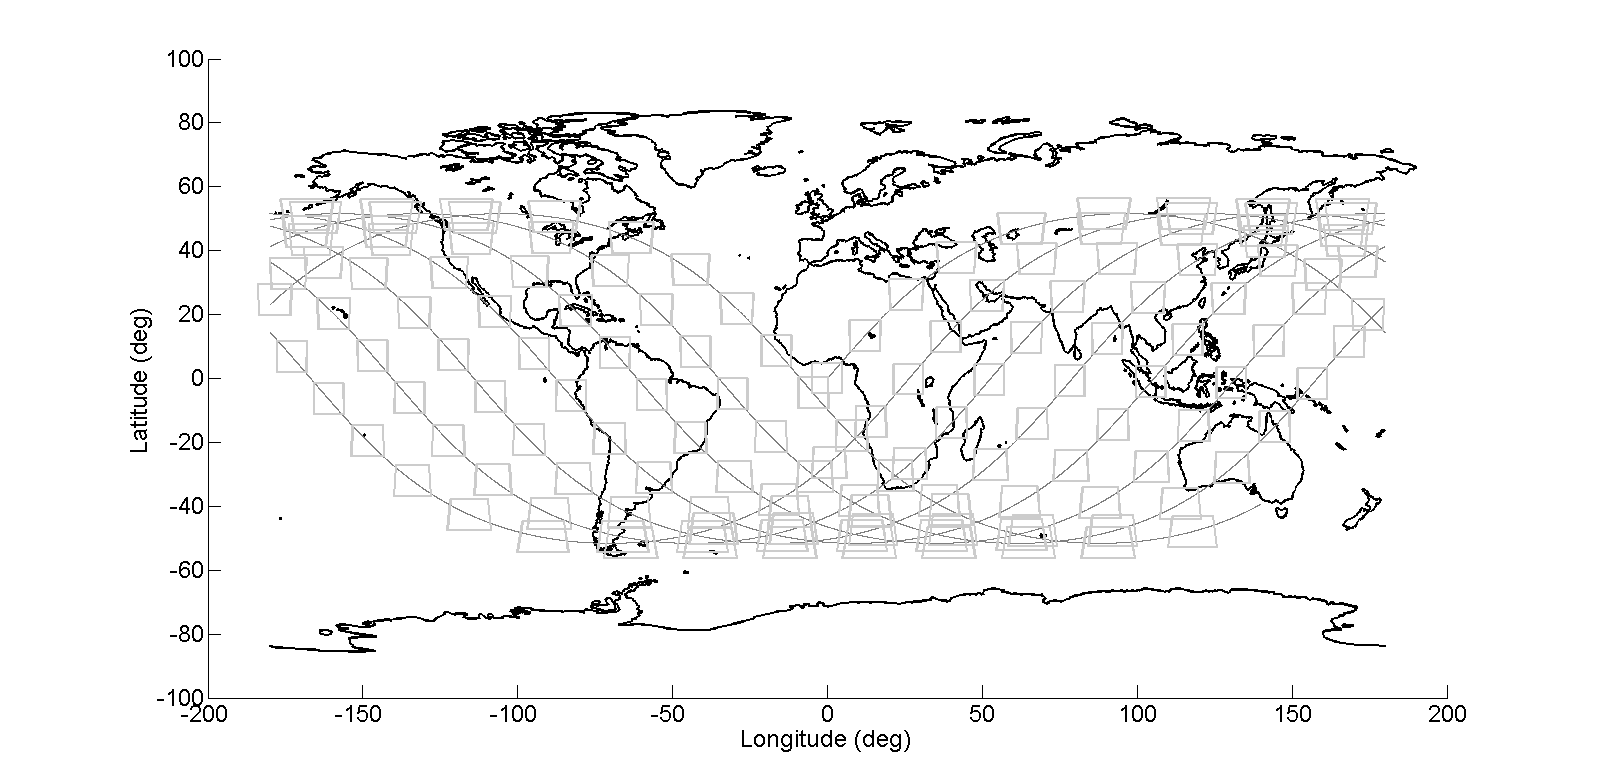
\includegraphics[width=0.95\textwidth]{ISScoverage} %lbrt
\caption{Coastlines visible from a spacecraft in a 56\degree inclination and 1000 km circular orbit with images taken once every 5 minutes}
\label{fig:coverage}
\end{figure}
%
The ground projected field-of-view (GFOV) can be calculated based on the geometry of the spacecraft position and desired field-of-view (FOV) of the camera,
%
\begin{equation}
GFOV=2h\tan\left(\frac{FOV}{2}\right)
\label{eq:GFOV}
\end{equation}
%
where $h$ is the spacecraft altitude.  A $30\degree$ FOV was chosen resulting in a viewable footprint of approximately 536 km.  A visual representation of the relative size of this footprint as seen by a camera can be seen in Fig.~\ref{fig:satellite} which shows a portion of the Great Lakes.
%
\begin{figure}[h!]
\centering
\begin{subfigure}{.48\textwidth}
  \centering
  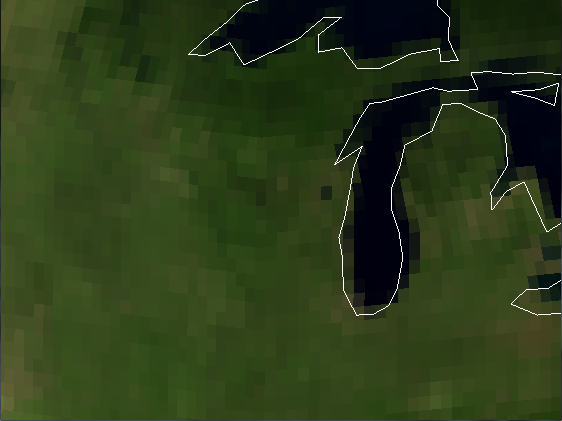
\includegraphics[width=0.9\textwidth]{Michigan_sat}
  \caption{Simulated satellite image incorporating a camera with a 30\degree FOV in a 1000 km circular polar orbit.  The blue lines represent the coastline data provided by MATLAB.}
  \label{fig:satellite}
\end{subfigure}\hfill
\begin{subfigure}{.48\textwidth} 
  \centering
  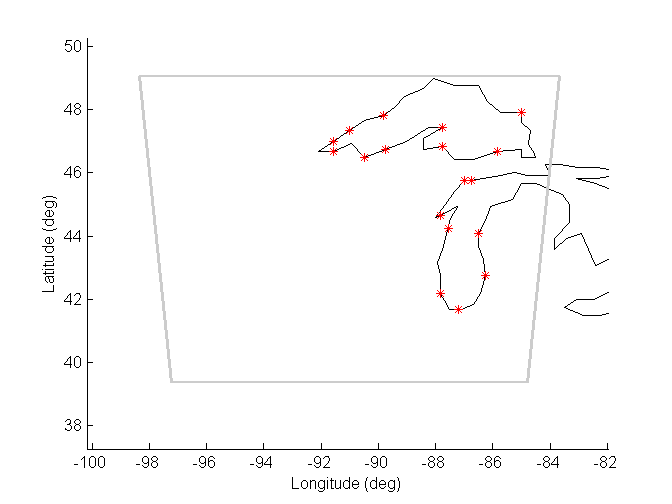
\includegraphics[width=0.9\textwidth]{Michigan}
  \caption{View of MATLAB coastlines showing exact footprint with various identified coastline points (*) within the spacecraft FOV}
  \label{fig:coastline}
\end{subfigure}
%\caption{View of MATLAB coastlines showing exact footprint with various identified coastline points (*) within the spacecraft FOV}
\label{fig:matlabstuff}
\end{figure}
%
%
%\begin{figure}[t!]
%\centering
  %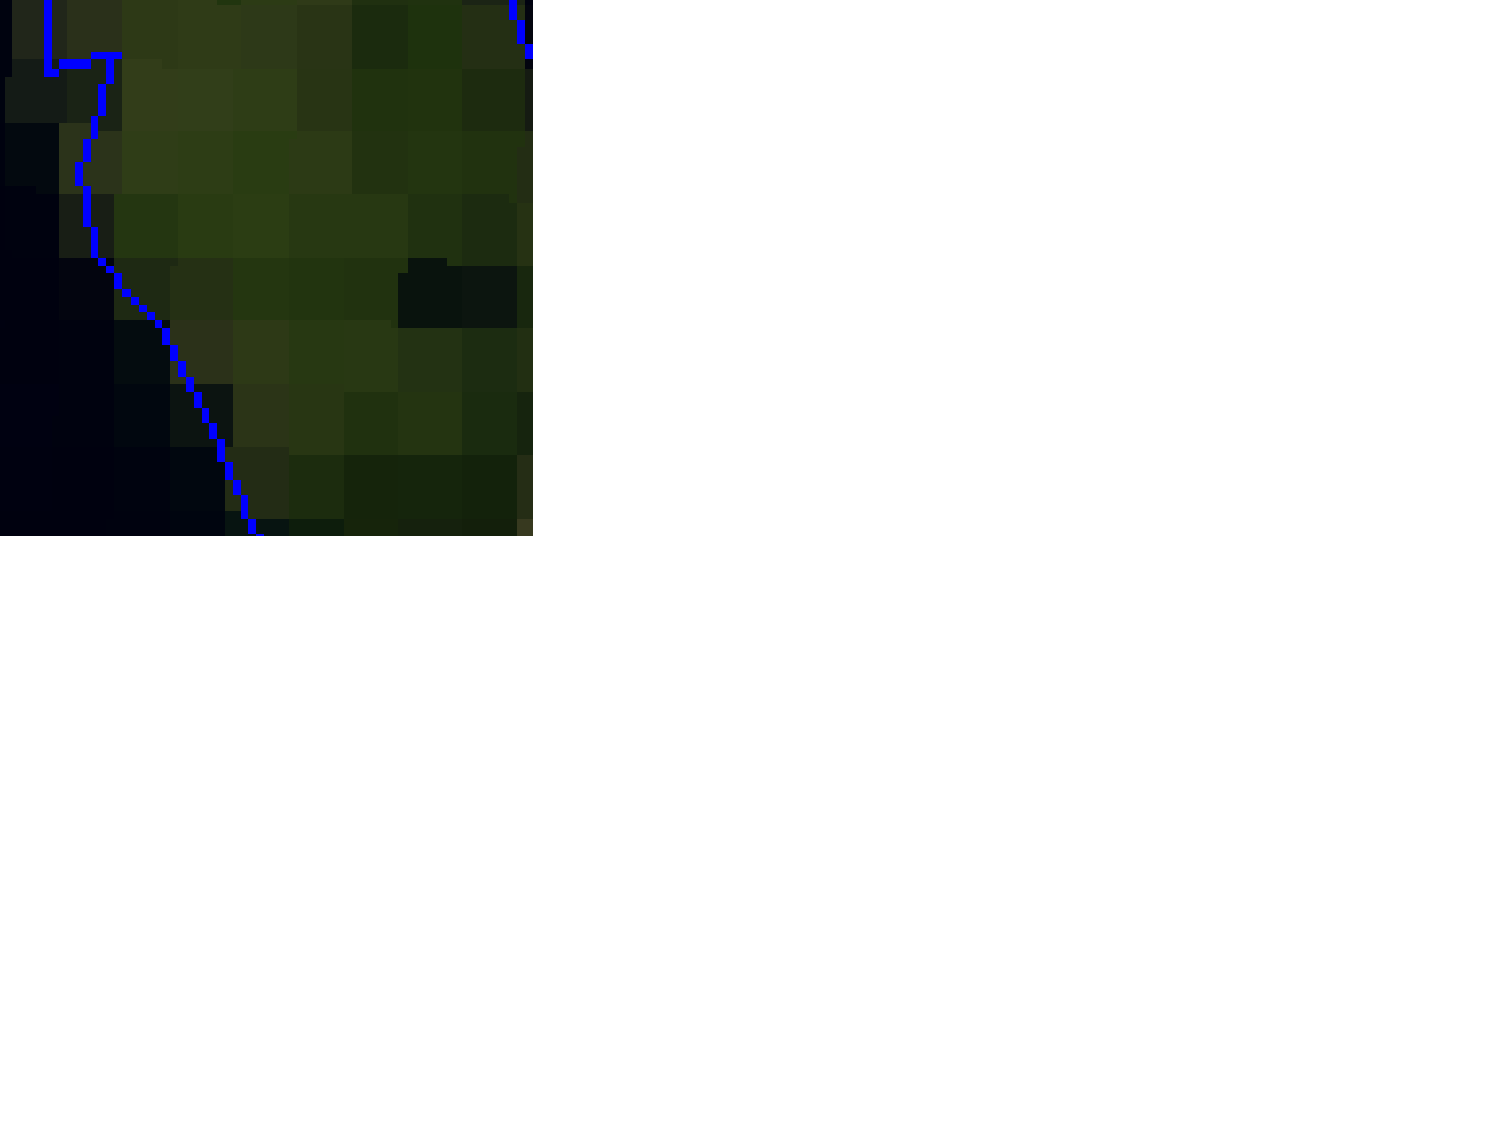
\includegraphics[width=.25\linewidth,trim=0in 3.8in 6.3in 0in,clip]{30FOV.pdf} %lbrt
  %\caption{Satellite image with a $30\degree$ FOV.}
  %\label{fig:fovimage}
%\end{figure}
%

%%%%%%%%%%%%%%%%%%%%%%%%%%%%%%%%%%%%%%%%%%%%%%%%%%%%%%%%

\section{Mathematical Models}
In order to create an algorithm for optical navigation, it is necessary to understand the mathematical models describing the state of the spacecraft as well as the camera model.  These models are described in the following sections.

%%%%%%%%%%%%%%%%%%%%%%%%%%%%%%%%%%%%%%%%%%%%%%%%%%%%%%%%

\subsection{Extended Kalman Filter}
Due to the nonlinear nature of spacecraft dynamics and optical measurements, an Extended Kalman Filter (EKF) will be used to estimate the state of the system \cite{Gelb,KalmanFiltering}.  The key equations are now briefly reviewed.

Suppose we have a nonlinear system governed by 
%
\begin{equation}
\label{eq:F}
\dot{\textbf{x}}=\textbf{f}(\textbf{x},t)+\textbf{v}
\end{equation}
%
where \textbf{v} is zero mean white noise.  The covariance of such a system may be propagated by 
%
\begin{equation}
\label{eq:Pdot}
\dot{\textbf{P}}=\textbf{F}\textbf{P}+\textbf{P}\textbf{F}^T+\textbf{Q}
\end{equation}
%
where 
%
\begin{equation}
\label{eq:F}
\textbf{F}(t)=\frac{\partial{\textbf{f}(\textbf{x},t)}}{\partial{\textbf{x}}}\Big{|}_{\textbf{x}=\hat{\textbf{x}}}
\end{equation}
%
Further suppose that at some time, $t_{k}$, a new measurement becomes available that is described by 
%
\begin{equation}
\label{eq:ymeas}
\tilde{\textbf{y}}_k=\textbf{h}(\textbf{x}_k)+\textbf{u}_k
\end{equation}
%
where $\textbf{u}_k \sim \mathcal{N}(0,\textbf{R}_k)$ and $\textbf{h}(\textbf{x})$ is the nonlinear measurement model, described in detail in Section \ref{ref:MeasModel}.
%\begin{equation}
%\label{eq:xdot}
%\dot{\textbf{x}}=\textbf{f}(\hat{\textbf{x}},t)
%\end{equation}
%
%\begin{equation}
%\label{eq:bigH}
%\textbf{H}_i\triangleq\frac{\partial{h(\textbf{x})}}{\partial{\textbf{x}}}\Big{|}_{\textbf{x}=\hat{\textbf{x}}}
%\end{equation}
%

Both the \textit{a posteriori} state and covariance estimates, $\hat{\textbf{x}}_k^+$ and $\textbf{P}_k^+$, may now be computed by
%
\begin{equation} \label{eq:xhatplus}
\hat{\textbf{x}}_k^+=\hat{\textbf{x}}_k^-+\textbf{K}_k(\tilde{\textbf{y}}_k-\textbf{h}(\hat{\textbf{x}}_k^-))
\end{equation}
%
\begin{equation} \label{eq:Pplus}
\textbf{P}_k^+=(\textbf{I}-\textbf{K}_k\textbf{H}_k)\textbf{P}_k^-(\textbf{I}-\textbf{K}_k\textbf{H}_k)^T+\textbf{K}_k\textbf{R}_k\textbf{K}_k^T
\end{equation}
%
where $\textbf{H}_k$ is the measurement sensitivity matrix,
%
\begin{equation} \label{eq:Jacobian}
\textbf{H}_k\triangleq\frac{\partial{\textbf{h}(\textbf{x})}}{\partial{\textbf{x}}}\Big{|}_{\textbf{x}=\hat{\textbf{x}}}
\end{equation}
%
Finally, the optimal update is achieved when $\textbf{K}_k$ is chosen to be the Kalman gain, where
%
\begin{equation} \label{eq:K}
\textbf{K}_k=\textbf{P}^-\textbf{H}_k^T(\textbf{H}_k\textbf{P}\textbf{H}_k^T+\textbf{R}_k)^{-1}
\end{equation}
%

%%%%%%%%%%%%%%%%%%%%%%%%%%%%%%%%%%%%%%%%%%%%%%%%%%%%%%%%

\subsection{State Propagation using an Extended Kalman Filter}
To estimate the state of the spacecraft, the dynamics can be expressed using two-body problem orbital mechanics.  The resulting equations of motion for the spacecraft are described by
%
\begin{equation} \label{eq:TwoBodyEq}
\ddot{\textbf{r}}=\frac{-\mu}{\|\textbf{r}\|^{3}}\textbf{r}
\end{equation}
%
Rewriting in state-space form leads to the following expression for $\textbf{f}(\textbf{x},t)$
%
\begin{equation} \label{eq:x}
\textbf{x}=
\left[\begin{matrix}
\textbf{r} \\
\dot{\textbf{r}}\end{matrix}\right]
\end{equation}
\quad \quad \quad
%
\begin{equation} \label{eq:TwoBodyEqMatrix}
\textbf{f}(\textbf{x},t)=
\left[\begin{matrix}
{\dot{\textbf{r}}} \\
\frac{-\mu}{{\|\textbf{r}\|^{3}}}\textbf{r}
\end{matrix}\right]
\end{equation}
%
Because $\ddot{\textbf{r}}$ is nonlinear in $\textbf{r}$, $\dot{\textbf{x}}$ must be linearized to first order about the estimate to find $\textbf{F}(t)$,
%
\begin{equation} \label{eq:Fmat}
\textbf{F}(t)=\frac{\partial{\textbf{f}(\textbf{x},t)}}{\partial{\textbf{x}}}\Big{|}_{\textbf{x}=\hat{\textbf{x}}}=
\left[\begin{matrix}
\frac{\partial{\dot{\textbf{r}}}}{\partial{\textbf{r}}} & \frac{\partial{\dot{\textbf{r}}}}{\partial{\dot{\textbf{r}}}} \\[0.4em]
\frac{\partial{\ddot{\textbf{r}}}}{\partial{\textbf{r}}} & \frac{\partial{\ddot{\textbf{r}}}}{\partial{\dot{\textbf{r}}}} \\
\end{matrix}\right]=
\left[\begin{matrix}
0_{3\times3} & \textbf{I}_{3\times3} \\
\frac{-\mu}{\|\hat{\textbf{r}}\|^3}\textbf{I}_{3\times3}+\frac{-\mu}{\|\hat{\textbf{r}}\|^5}\hat{\textbf{r}}\hat{\textbf{r}}^T & 0_{3\times3} \\[0.4em]
\end{matrix}\right]
\end{equation}
%
Since both $\dot{\textbf{x}}$ and $\dot{\textbf{P}}$ are now known, each can be integrated to propagate to a new \textit{a priori} estimate of the state and covariance, $\hat{\textbf{x}}_k^-$ and $\hat{\textbf{P}}_k^-$, which are then updated by the EKF.

%%%%%%%%%%%%%%%%%%%%%%%%%%%%%%%%%%%%%%%%%%%%%%%%%%%%%%%%

\subsection{Measurement Model for Coastline Points in Images} \label{ref:MeasModel}
Line-of-sight (LOS) measurements are produced by the images obtained from the spacecraft's camera.  However, these measurements produce a nonlinear function of the spacecraft state and may be determined by the geometry between the Earth and the spacecraft as shown in Fig. \ref{fig:LOSgeometry}.  From this figure, it is clear that the following geometric relations are obtained by
%
\begin{figure}[ht!]
\centering
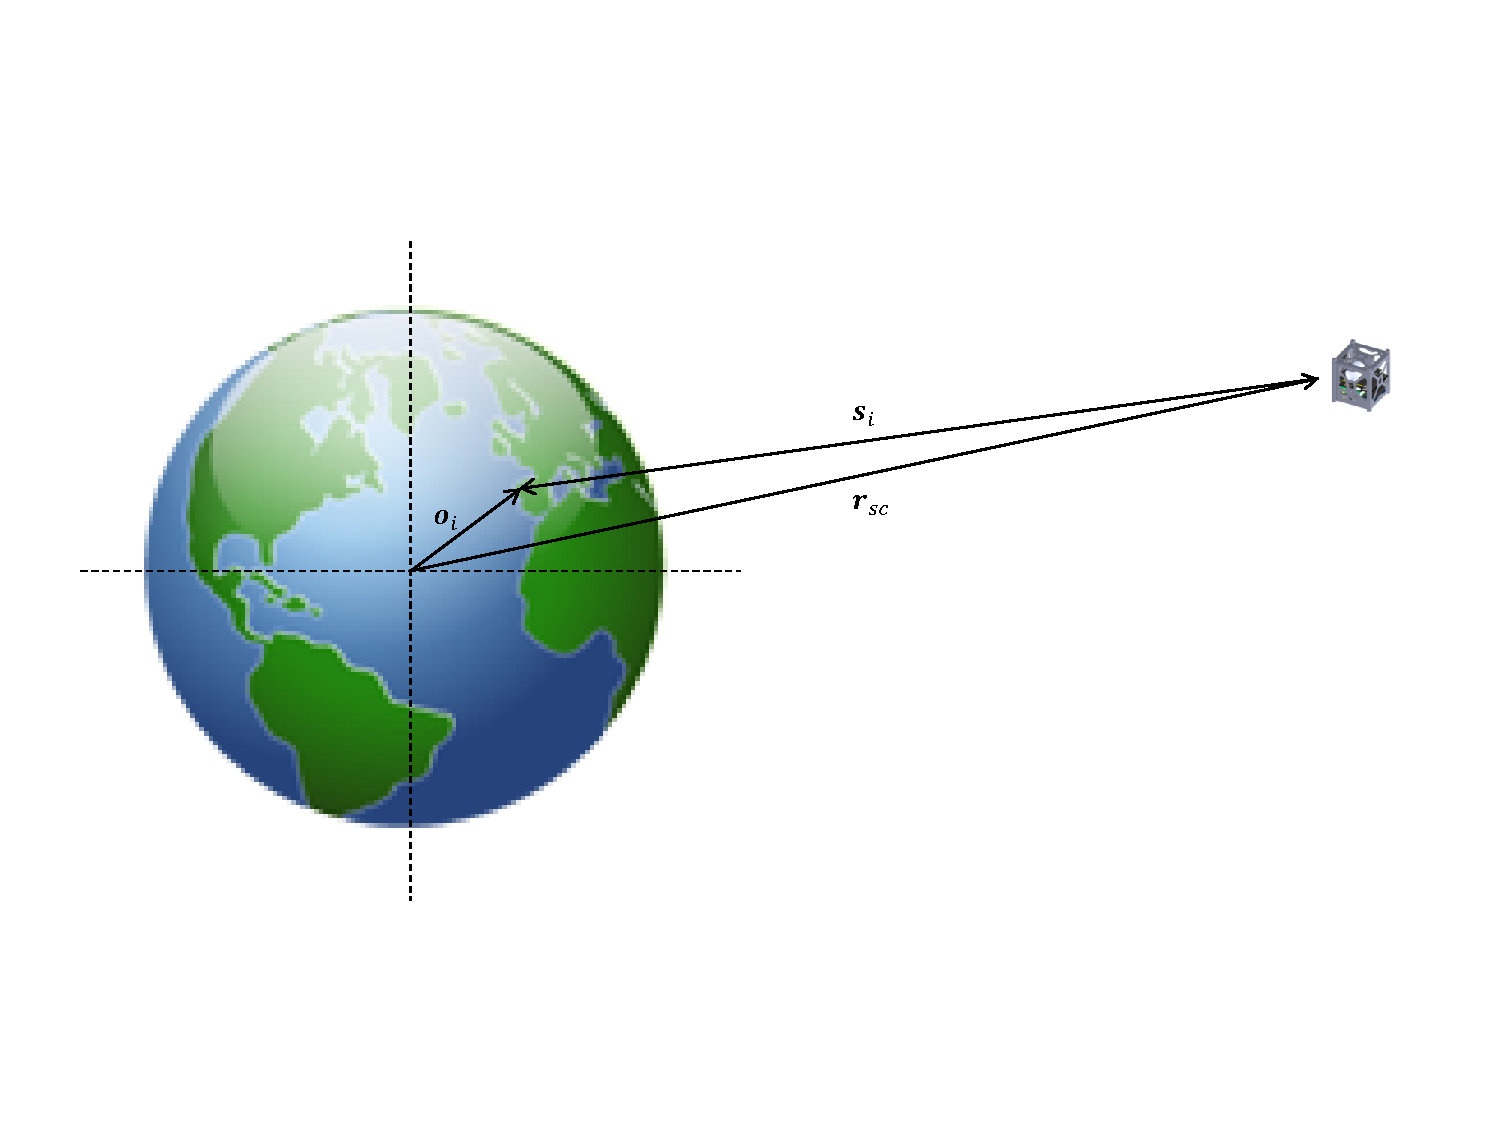
\includegraphics[width=0.75\textwidth,trim=0.8in 1.5in 0.3in 1in,clip]{LOSgeometry} %lbrt
\caption{Line-of-sight vectors for measurement model}
\label{fig:LOSgeometry}
\end{figure}
%
\begin{equation} \label{eq:s}
\textbf{s}_i=\textbf{o}_i-\textbf{r}_{sc}
\end{equation}
%
\begin{equation} \label{eq:eii}
\textbf{e}_{iI}=\frac{\textbf{s}_i}{\|\textbf{s}_i\|}
\end{equation}
%
where $\textbf{r}_{sc}$ is the position of the spacecraft from the center of the earth, $\textbf{s}_i$ is the vector from the spacecraft to the $i^{th}$ observed point, or landmark, and $\textbf{o}_i$ is the vector from the center of the earth to the landmark.  The measurement model for a single observed coastline point can then be described as
%
\begin{equation} \label{eq:littleh}
\textbf{h}(\textbf{x})=\textbf{e}_{iC}=\textbf{T}_{C}^I\textbf{e}_{iI}=\textbf{T}_{C}^I\frac{\textbf{s}_i}{[\textbf{s}_i^T\textbf{s}_i]^{1/2}}
\end{equation}
%
where $\textbf{T}_C^I$ is the rotation matrix from the inertial frame to the camera frame.  From here, the measurement sensitivity matrix may be computed as
%
\begin{equation}
\label{eq:H}
\textbf{H}_{i}=\textbf{T}_{C}^I\frac{1}{\|\textbf{s}_i\|}
\left[\begin{matrix}
\{\textbf{e}_{iI}\textbf{e}_{iI}^T-\textbf{I}_{3\times3}\} & \textbf{0}_{3\times3}
\end{matrix}\right]
\end{equation}
%
It should be noted that in order to calculate the Kalman gain, as seen in Eq.~\ref{eq:K}, the quantity $\textbf{H}_i\textbf{P}\textbf{H}_i^T+\textbf{R}_i$ must be invertible.  In this particular case, the null space of the measurement covariance, $\textbf{R}_{i}$ is the same as the null space of $\textbf{H}_i\textbf{P}\textbf{H}_i^T$ assuming $\textbf{R}_i$, is determined to first order using the QUEST covariance matrix, as is common practice with unit vector measurements \cite{Shuster:1981}.
%
\begin{equation}\label{eq:meascovR}
\textbf{R}_{i}=E[(\textbf{e}_{iC}-\bar{\textbf{e}}_{iC})(\textbf{e}_{iC}-\bar{\textbf{e}}_{iC})^T]\approx\sigma_\Theta^2(\textbf{I}_{3\times3}-\bar{\textbf{e}}_{iC}\bar{\textbf{e}}_{iC}^T)
\end{equation}
%which causes the matrix to be non-invertible (a $3\times3 $ matrix with rank 2).  To avoid numerical issues in calculations, the Kalman gain equation can be adjusted by adding a rank-one matrix where $\nu\textbf{e}_i\textbf{e}_i^T$ \cite{Liounis:2013}.
%
\begin{equation} \label{eq:Knew}
\textbf{K}_i=\textbf{P}^-\textbf{H}_i^T(\textbf{H}_i\textbf{P}\textbf{H}_i^T+\textbf{R}_i+\nu\textbf{e}_i\textbf{e}_i^T)^{-1}
\end{equation}

%
It should also be noted that in Eq. \ref{eq:K}, $\nu=0.5tr[\textbf{R}_i]$ is chosen to ensure the matrix we are inverting is well conditioned. As explained in [\citen{Liounis:2013}], this does not change the value of $\textbf{K}_i$ since it is equivalent to adding a $\textbf{0}$ to the overall equation,
%
\begin{equation} \label{eq:Htranse}
\textbf{H}_i^T\textbf{e}_i=0
\end{equation}
%

%%%%%%%%%%%%%%%%%%%%%%%%%%%%%%%%%%%%%%%%%%%%%%%%%%%%%%%%

\section{Results}
For this simulation, it is important to ensure that coastlines will be visible based on the spacecraft's orbit and camera parameters.  Therefore, simulations were run to determine the percentage of time coastlines would be visible from the spacecraft's position in a 1000 km circular orbit with varying inclinations.  For simplicity, other orbital parameters, including the right ascension of the ascending node, the argument of periapsis, and the true anomaly, were fixed at 0 radians.  Fig.~\ref{fig:contourplot} shows the results of the simulations given various inclinations camera FOV.  It is important to note that these results are orbit-specific and will vary slightly due to differences in orbital parameters specific to a satellite's orbit. Consequently, the rate at which images are captured also plays a key role in determining how often coastlines are observable.  In this case, images are to be taken once every 30 seconds for a total of 24 hours.
\begin{figure}[ht!]
\centering
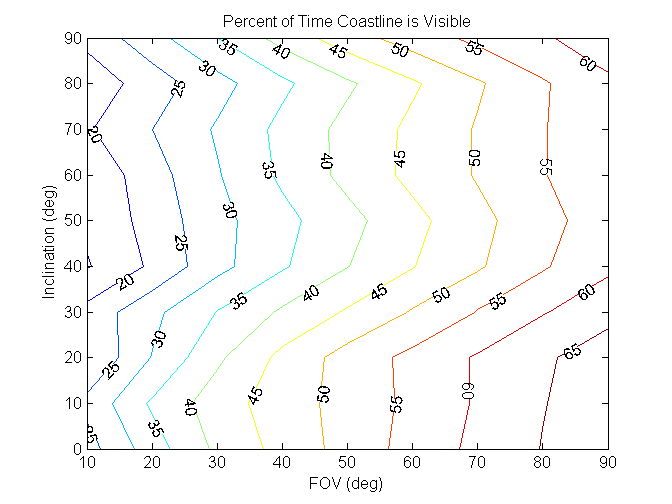
\includegraphics[width=0.75\textwidth]{contourplot} %lbrt
\caption{Orbit-specific contour plot showing the percentage of time coastline is observable based on inclination and FOV at a 1000 km circular orbit with images taken once every five minutes.}
\label{fig:contourplot}
\end{figure}

%%%%%%%%%%%%%%%%%%%%%%%%%%%%%%%%%%%%%%%%%%%%%%%%%%%%%%%%
\subsection{Assessment of Navigation Filter Performance}
Monte Carlo analyses were run for three different inclinations: 0\degree, 45\degree, and 90\degree.  As seen in Fig.~\ref{fig:mcpos0}, the error between the predicted and true values all lie within the 3$\sigma$ bounds of the covariance, meaning the position of the spacecraft can be estimated to within a few meters of the true position while the velocity can be estimated to within a few millimeters of the true velocity.  
\begin{figure}[ht!]
\centering
\begin{subfigure}{.5\textwidth}
  \centering
  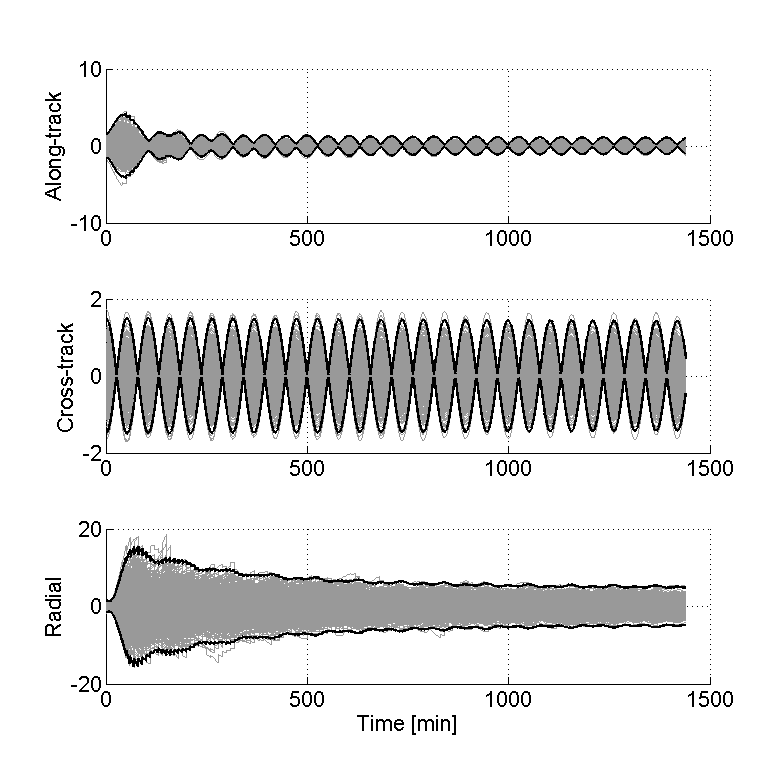
\includegraphics[width=0.9\linewidth]{MC_pos0}
  \caption{Position Error [m] at i=0\degree}
  \label{fig:mcpos0}
\end{subfigure}%
\begin{subfigure}{.5\textwidth} 
  \centering
  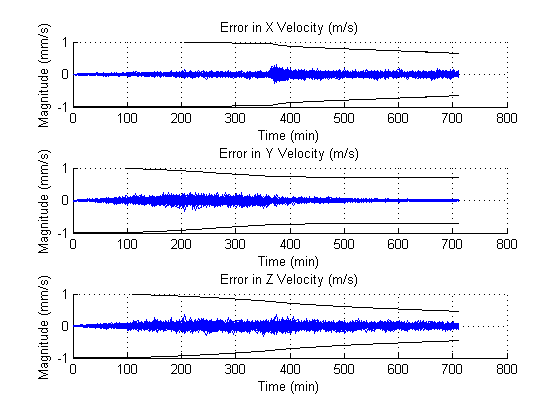
\includegraphics[width=0.9\linewidth]{MC_vel0}
  \caption{Velocity Error [mm/s] at i=0\degree}
  \label{fig:coastline}
\end{subfigure}
\caption{Monte Carlo Position and Velocity Errors at 1000 km polar orbit}
\label{fig:mcvel0}
\end{figure}
%
Comparing Fig.~\ref{fig:mcpos0} through Fig.~\ref{fig:mcvel90}, it is apparent where measurements are not present, i.e. where the camera cannot detect coastlines.  In all orbits, measurements appear to be available when images are taken every 30 seconds, hence the constant convergence of the covariance towards steady state.  
\begin{figure}[ht!]
\centering
\begin{subfigure}{.5\textwidth}
  \centering
  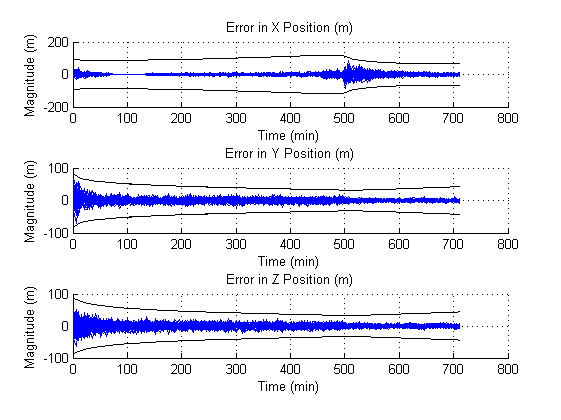
\includegraphics[width=0.9\linewidth]{MC_pos45}
  \caption{Position Error [m] at i=45\degree}
  \label{fig:mcpos45}
\end{subfigure}%
\begin{subfigure}{.5\textwidth} 
  \centering
  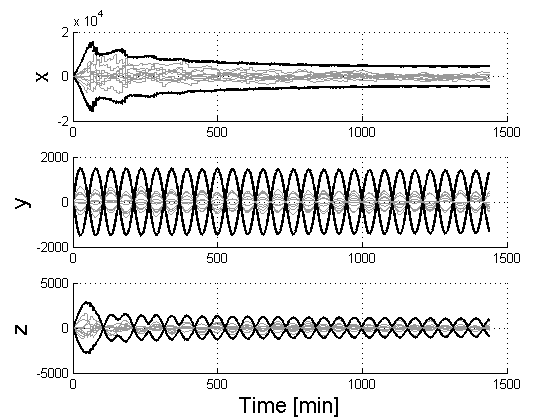
\includegraphics[width=0.9\linewidth]{MC_vel45}
  \caption{Velocity Error [mm/s] at i=45\degree}
  \label{fig:coastline}
\end{subfigure}
\caption{Monte Carlo Position and Velocity Errors at 1000 km 45 \degree orbit}
\label{fig:mcvel45}
\end{figure}
%
\begin{figure}[ht!]
\centering
\begin{subfigure}{.5\textwidth}
  \centering
  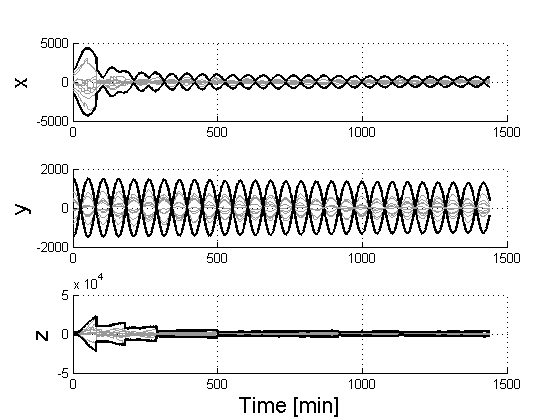
\includegraphics[width=0.9\linewidth]{MC_pos90}
  \caption{Position Error [m] at i=90\degree}
  \label{fig:mcpos90}
\end{subfigure}%
\begin{subfigure}{.5\textwidth} 
  \centering
  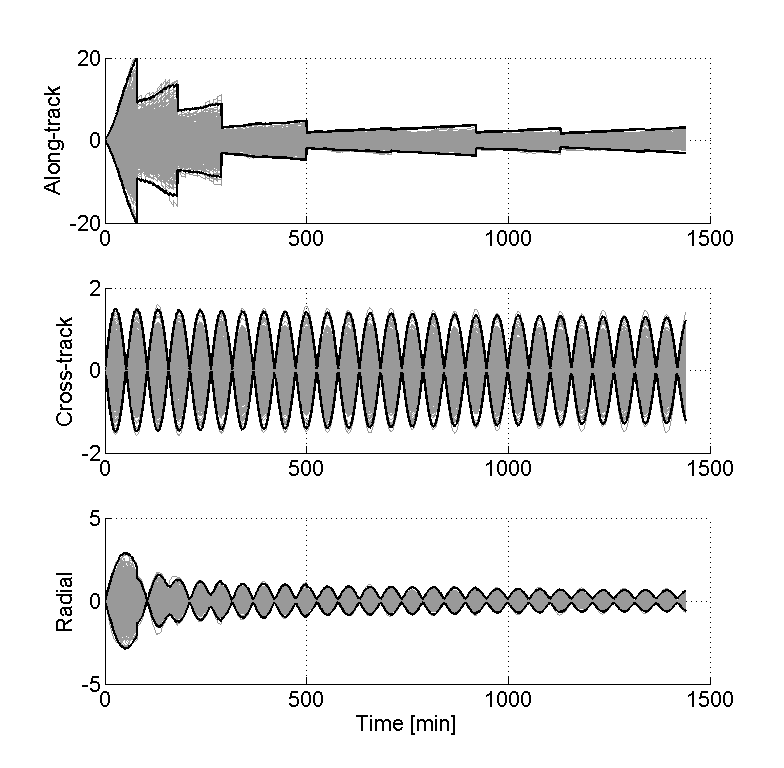
\includegraphics[width=0.9\linewidth]{MC_vel90}
  \caption{Velocity Error [mm/s] at i=90\degree}
  \label{fig:coastline}
\end{subfigure}
\caption{Monte Carlo Position and Velocity Errors at 1000 km 90 \degree orbit}
\label{fig:mcvel90}
\end{figure}
%
\section{Conclusion}
An Extended Kalman Filter was used to determine the accuracy in which a spacecraft's position and velocity can be determined through LOS vectors produced through coastline determination.  If a coastline is visible, an image processing algorithm is able to match it with a database that can calculate spacecraft position coordinates for each observed landmark.  These coordinates are input into the filter to determine the spacecraft's position and velocity within a maximum of 5 m and 5 mm/s, respectively.  Future work related to this topic includes creating an appropriate image processing algorithm able to extract the required information from sample satellite images.  It is hoped that this can be implemented on-board a CubeSat launched as part of West Virginia University's proposed WATSON (WVU Advanced Technology Satellite for Optical Navigation) CubeSat mission in the near future.
%
\section{Acknowledgments}
The authors thank Andrew Liounis of West Virginia University and Allison Willingham of NASA Goddard Space Flight Center for valuable feedback on this manuscript. This work was made possible by a NASA West Virginia Space Grant Consortium (WVSGC) 2014-2015 Research Initiation Grant. 

%%%%%%%%%%%%%%%%%%%%%%%%%%%%%%%%%%%%%%%%%%%%%%%%%%%%%%%%
\bibliographystyle{aiaa}
\bibliography{LitReviewSources}
\end{document}

% - Release $Name:  $ -